\documentclass[10pt,twocolumn,letterpaper]{article}

\usepackage{statcourse}
\usepackage{times}
\usepackage{epsfig}
\usepackage{graphicx}
\usepackage{amsmath}
\usepackage{amssymb}

% Include other packages here, before hyperref.

% If you comment hyperref and then uncomment it, you should delete
% egpaper.aux before re-running latex.  (Or just hit 'q' on the first latex
% run, let it finish, and you should be clear).
\usepackage[breaklinks=true,bookmarks=false]{hyperref}


\statcoursefinalcopy


\setcounter{page}{1}
\begin{document}


%%%%%%%%%%%%%%%%%%%%%%%%%%%%%%%%%%%%%%%%%%%%%%%%%%%%%%%%%%%%%%%
% DO NOT EDIT ANYTHING ABOVE THIS LINE
% EXCEPT IF YOU LIKE TO USE ADDITIONAL PACKAGES
%%%%%%%%%%%%%%%%%%%%%%%%%%%%%%%%%%%%%%%%%%%%%%%%%%%%%%%%%%%%%%%



%%%%%%%%% TITLE
\title{Midterm Project Report for Newspaper Bias project}

\author{Tom Arend\\
{\tt\small t.arend@phd.hertie-school.org}
\and
Nicolai Berk\\
{\tt\small nicolai.berk@gmail.com}
}

\maketitle
%\thispagestyle{empty}


% MAIN ARTICLE GOES BELOW
%%%%%%%%%%%%%%%%%%%%%%%%%%%%%%%%%%%%%%%%%%%%%%%%%%%%%%%%%%%%%%%

%%%%%%%%% ABSTRACT
\begin{abstract}
   Newspapers are one of the most important institutions in contemporary democracies. They have the power to affect voting behaviour, as well as polarise the electorate or motivate them to turn out to vote. Therefore, it is surprising that few papers deploy sate-of-the-art Deep Learning technologies to classify ideological bias in news articles. We apply a transformer neural network to classify party press releases by authorship. This model is then applied and optimised to estimate ideological bias in news articles. We fine-tune and validate the model using op-eds by politicians and compare pre-trained model to a BERT model that was not fine-tuned on party press releases. This approach provides a novel way to train powerful models on political language with scarce training data.\footnote{GitHub repository: \url{https://github.com/nicolaiberk/nlpdl\_project}}
\end{abstract}


%%%%%%%%% BODY TEXT

% \begin{itemize}
% {\color{blue}

% \item Remember that you should \textbf{submit the report}  via Moodle and \textbf{include in the report the link to accessible GitHub repository that contains the code}. Also, \textbf{only one member per team} needs to submit the project material. You must include a link to your GitHub repository for the project as the first footnote on the first page. 

% \item The midterm project report should be {\bf 4 pages long (not counting references), and a maximum 10 references}. The report should contain the sections that are already provided in this paper. It forms the basis of the final report with the same structure. Please check out the text in these sections for further information.

% \item Your midterm milestone will be graded on the following criteria:
% \begin{itemize}
% \item Progress: Has the team made good progress on the project? You should have done approximately half of the work of your project.
% \item As a minimum, your milestone should show that you have setup your data, baseline model code, and evaluation metric, and run experiments to obtain some results (assuming you are doing a typical model-building project). Other than this, `good progress' depends on various factors (e.g., whether your model is implemented from scratch or based on an existing codebase).
% \item Understanding: Does the milestone show a strong understanding of its problem, tasks, methods, metrics, and research context?
% \item Writing quality: Does the milestone clearly communicate what you've done and why, providing the requested information, to an appropriate level of detail (given the page limit)?
% \item You will receive some brief feedback on your milestone. Feedback may contain helpful suggestions for your project (e.g., try a particular method, read a particular paper) and/or warnings about your project plan (e.g., if your plans are too ambitious or not ambitious enough), and how you could improve your technical writing (e.g., adjustments to clarity, level of detail, formatting, use of references).
% \end{itemize}

% \item Technical writing is an important skill in this class, in research, and beyond. It's well worth spending time developing your ability to communicate technical concepts clearly. Here are some resources which might help you improve your technical writing:
% \begin{itemize}
% \item Tips for Writing Technical Papers, Jennifer Widom (\url{https://cs.stanford.edu/people/widom/paper-writing.html}).
% \item Write the Paper First, Jason Eisner (\url{https://www.cs.jhu.edu/~jason/advice/write-the-paper-first.html}).
% \end{itemize}

% \item Here are some other things you can do to improve your technical writing:
% \begin{itemize}
% \item Look carefully at several ML / NLP papers to understand their typical structure, writing style, and the usual content of the different sections. Model your writing on these examples.
% \item Think about the NLP / ML papers you've read (for example, the one you summarised for your proposal). Which parts did you find easy to understand and why? Which parts did you find difficult to understand and why? Can you identify any good writing practices that you could use in your technical writing?
% \item Ask a friend to read through your writing and tell you if is clear. This can be useful even if the friend does not have the relevant technical knowledge.
% \end{itemize}
% }
% \end{itemize}

\section{Proposed Method}



% This section details your approach(es) to the problem. For example, this is where you describe the architecture of your model, and any other key methods or algorithms.

% You should also describe your baseline(s). Depending on space constraints, and how standard your baseline is, you might do this in detail, or simply refer the reader to some other paper for the details. 

% If any part of your approach is original, make it clear (so we can give you credit!). For models and techniques that aren't yours, provide references.

% If you're using any code that you didn't write yourself, make it clear and provide a reference or link. When describing something you coded yourself, make it clear (so we can give you credit!).

The measurement of ideology and political bias are the subject of much research on political text \cite{X,Y,Z}. However, researchers often find themselves facing a lack of appropriate training data. Manual annotation is usually costly and so it might be useful to infer ideology from other sources of text.

We test this reasoning for the measurement of newspaper bias. We measure newspaper bias as an articles similarity to a given parties' communication. Using pre-trained BERT neural network models for German language\footnote{[link to huggingface model]} (\cite{BERTPaper}), we compare how three different training processes affect model performance. We expect optimal performance from a transformer neural network fine-tuned in two steps: first, for classification of party press releases by authorship. This model is then applied and optimised to estimate ideological bias in news articles by fine-tuning and validating the model using op-eds by politicians. We compare this fine-tuned model to a BERT model that was not fine-tuned on party press releases and one that was not fine-tuned on newspaper data. This leaves us with three models:

\begin{enumerate}
    \item A model fine-tuned on a limited amount of newspaper articles authored by politicians.
    \item A model fine-tuned on party press releases.
    \item A model both fine-tuned on press releases and politicians' newspaper contributions.
\end{enumerate}

This way, we can assess how much model performance is improved when including information from both party press releases and newspaper data.

\section{Experiments}

\paragraph{Data:} In this project, we draw on three data sources:
\begin{itemize}
    \item A dataset of over 40,000 German party press releases collected by the SCRIPTS project (\cite{}) for training.
    \item A collection of over 2 million German newspaper articles collected by one of the authors in a previous project (\cite{}).
    \item A collection of German newspaper articles authored by politicians collected as part of this project.
\end{itemize}

\paragraph{Evaluation method:} So far, we have successfully fine-tuned a BERT-model to classify party-press releases by authorship (model 2, serving as the basis for model 3). The performance of this model can be seen in \ref{fig:party}. As the reader can see, the model shows a near-perfect classification performance. This was rather surprising to the authors and shifted the initial focus of the project from improving the classification of party press releases to improving the performance on newspaper articles.

\begin{figure}
    \centering
    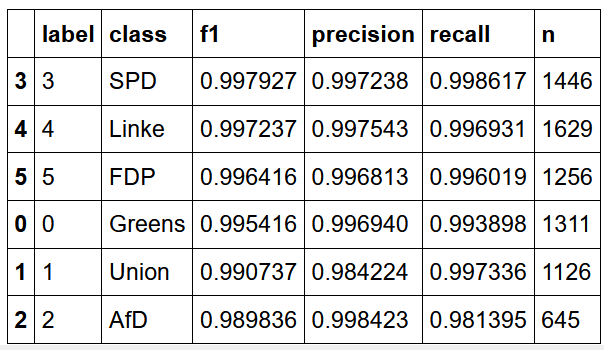
\includegraphics[width=0.4\textwidth]{reports/midterm-report-latex/figures/party_class.png}
    \caption{Performance of model 2 for the classification of party press releases.}
    \label{fig:party}
\end{figure}

For the final assessment of classifier performance, we will predict the author's party of newspaper articles from politicians. This way, we can use the party labels from earlier fine-tuning exercises in the assessment of newspaper bias. As we aim for a balance of precision and recall, we will evaluate the models' F1-score. Additionally, we will assess generalisability by assessing the placement of newspapers - left-wing newspapers such as the TAZ should be placed closer to left-wing parties (Grüne, SPD, Linke) than right-wing newspapers (FAZ, WELT).

\paragraph{Experimental details:} How you ran your experiments (e.g. model configurations, learning rate, training time, etc.)



\paragraph{Results:} We classified a training set of 4,000 newspaper articles using model 2 (fine-tuned on party press releases). We expected articles from conservative newspapers FAZ and Welt to be more similar to Union and FDP and possibly the AfD, especially compared to the progressive TAZ. Spiegel Online (SPON) is expected to be equally similar to right- and leftwing newspapers.

The results can be seen in table \ref{tbl:means}, which shows the average probability for an article to be classified as being authored by a given party. As expected, FAZ and Welt are very similar to Union (81\%) and FDP (58\%/55\%), but also rather similar to the Greens (36\%/35\%). While they show the highest similarity to the AfD (8\%/7\%), similarity to the radical-right party is generally on a very low level among all newspapers. Spiegel Online (SPON) shows lower similarity to the FDP and closer to Union and Greens, but generally rather similar to the right-wing newspapers. The TAZ shows a comparatively different profile, being very similar to the greens (an average article is classified as being authored by the Grüne with 70\%), and less similar to the Union parties (41\%), the FDP (32\%), and the AfD (5\%). Surprisingly, it also shows the lowest similarity to the Linke (13\%). Maybe most surprising is the general low similarity to SPD press releases (4\%/5\%). It seems the party has a rather distinctive style in its press releases.

\begin{table}[!htbp] \centering 
    \begin{tabular}{@{\extracolsep{1pt}} lcccccc}
    \\[-1.8ex]\hline 
    \hline \\[-1.8ex] 
    Paper & Linke & Grüne & SPD & Union & FDP & AfD \\ 
    \hline \\[-1.8ex] 
    FAZ & $0.15$ & $0.36$ & $0.05$ & $0.81$ & $0.58$ & $0.08$ \\ 
    Welt & $0.15$ & $0.35$ & $0.05$ & $0.81$ & $0.55$ & $0.07$ \\ 
    Spiegel & $0.11$ & $0.39$ & $0.05$ & $0.89$ & $0.34$ & $0.07$ \\ 
    TAZ & $0.13$ & $0.69$ & $0.04$ & $0.41$ & $0.32$ & $0.05$ \\ 
    \hline \\[-1.8ex] 
    \end{tabular} 
  \caption{Mean similarity estimate to each party by newspaper.} 
  \label{tbl:means} 
\end{table}

Given that model 2 is the likely the worst performing, these are promising results. However, we need to look into the odd performance for the SPD.

\section{Future work}

\begin{itemize}
    \item Collect politicians op-eds (\& interviews?).
    \item Train model 1 and model 3 on the op-eds.
    \item Assess performance for each of these models.
\end{itemize}


{\small
\bibliographystyle{ieee}
\bibliography{bibliography.bib}
}

\end{document}
